\documentclass{article}
\usepackage[utf8]{inputenc}
\usepackage[T1]{fontenc}
\usepackage{graphicx}
\usepackage{amsmath, amssymb}
\usepackage{xcolor}
\usepackage{tikz}
\usepackage{lipsum}
\usepackage{sectsty}
\usepackage{enumerate}
\usepackage{pgfplots}

\title{Practice Questions}
\author{Hia Al Saleh}
\date{February 22nd, 2024}
\begin{document}
\maketitle
\section*{Chapter 1.3 \& 1.4}
Page 39, \#1, 2, 3, 6, 8, 13

\begin{itemize}
\item Question 1:
\begin{enumerate}
    \item 
    \begin{enumerate}
        \item $f(x) = (x - 4)(x + 3)(2x - 1)$
        \begin{itemize}
            \item i) The degree of $f(x)$ is 3 and the leading coefficient is positive.
            \item ii) As $x$ approaches negative infinity, $f(x)$ increases without bound, and as $x$ approaches positive infinity, $f(x)$ also increases without bound.
            \item iii) The x-intercepts are $x = 4$, $x = -3$, and $x = \frac{1}{2}$.
        \end{itemize}
        
        \item $g(x) = -2(x + 2)(x - 2)(1 + x)(x - 1)$
        \begin{itemize}
            \item i) The degree of $g(x)$ is 4 and the leading coefficient is negative.
            \item ii) As $x$ approaches negative infinity, $g(x)$ decreases without bound, and as $x$ approaches positive infinity, $g(x)$ decreases without bound.
            \item iii) The x-intercepts are $x = -2$, $x = 2$, $x = -1$, and $x = 1$.
        \end{itemize}
        
        \item $h(x) = (3x + 2)^2(x - 4)(x + 1)(2x - 3)$
        \begin{itemize}
            \item i) The degree of $h(x)$ is 5 and the leading coefficient is positive.
            \item ii) As $x$ approaches negative infinity, $h(x)$ increases without bound, and as $x$ approaches positive infinity, $h(x)$ also increases without bound.
            \item iii) The x-intercepts are $x = -\frac{2}{3}$, $x = -\frac{2}{3}$, $x = 4$, $x = -1$, and $x = \frac{3}{2}$.
        \end{itemize}
        
        \item $p(x) = -(x + 5)^3(x - 5)^3$
        \begin{itemize}
            \item i) The degree of $p(x)$ is 6 and the leading coefficient is negative.
            \item ii) As $x$ approaches negative infinity, $p(x)$ decreases without bound, and as $x$ approaches positive infinity, $p(x)$ decreases without bound.
            \item iii) The x-intercepts are $x = -5$ and $x = 5$.
        \end{itemize}
    \end{enumerate}
\end{enumerate}
\item Question 2:
a)
\begin{figure}[ht]
    \centering
    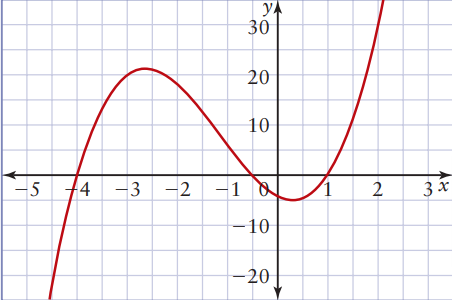
\includegraphics[width=0.6\textwidth]{imgs/ga.png}
\end{figure}

\begin{enumerate}[i.]
    \item -4, -0.5, 1
    \item $f(x)>0$\\$-4<x<-0.5, x>1$\\$x\in(-4,-0.5)\cup(1, \infty)$\\
          $f(x)<0$\\$x<-4$ or $-0.5<x<1$\\$x\in(-\infty,-4)\cup(-0.5, 1)$
    \item Order 1
\end{enumerate}
2b)
\begin{figure}[ht]
    \centering
    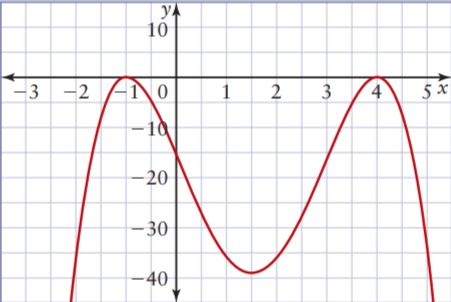
\includegraphics[width=0.6\textwidth]{imgs/gb.png}
\end{figure}

\begin{enumerate}[i.]
    \item -2, 4
    \item $f(x)<0$ when $\to x \in \mathbb{R}, x\neq-1,4$  \\ $x\in (-\infty,-1)\cup(-1,4)\cup(4,\infty)$
    \item Order 2
\end{enumerate}
2c)
\begin{figure}[ht]
    \centering
    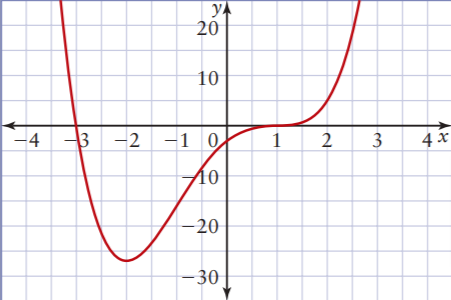
\includegraphics[width=0.6\textwidth]{imgs/gc.png}
\end{figure}

\begin{enumerate}[i.]
    \item x=-3,1
    \item $f(x)>0, x\in (-\infty,-3)\cup(1,\infty)$\\ $f(x)<0, x\in(-3,1)$
    \item Order 1
\end{enumerate}
2d)
\begin{figure}[ht]
    \centering
    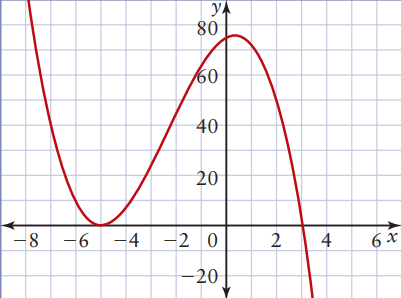
\includegraphics[width=0.6\textwidth]{imgs/gd.png}
\end{figure}

\begin{enumerate}[i.]
    \item x=-5,3
    \item $f(x)>0, x\in (-\infty,-5)\cup(-5,3)$\\ $f(x)<0, x\in(3,\infty)$
    \item Order 2
\end{enumerate}
\newpage

\item Question 3:\\
\begin{enumerate}
    \item 
    \begin{enumerate}
        \item 
        \begin{itemize}
            \item i) $f(x) = -2(x - 3)(x + 2)(4x - 3)$
            \item Zeros:
                \begin{itemize}
                    \item $x = 3$ of order 1
                    \item $x = -2$ of order 1
                    \item $x = \frac{3}{4}$ of order 1
                \end{itemize}
        \end{itemize}
        
        \item 
        \begin{itemize}
            \item ii) $g(x) = (x - 1)(x + 3)(1 - x)(3x - 9)$
            \item Zeros:
                \begin{itemize}
                    \item $x = 1$ of order 1
                    \item $x = -3$ of order 1
                    \item $x = 1$ of order 1
                    \item $x = 3$ of order 1
                \end{itemize}
        \end{itemize}
        
        \item 
        \begin{itemize}
            \item iii) $h(x) = -2(x + 4)^2(x - 1)^2(x + 2)(2x - 3)$
            \item Zeros:
                \begin{itemize}
                    \item $x = -4$ of order 2
                    \item $x = 1$ of order 2
                    \item $x = -2$ of order 1
                    \item $x = \frac{3}{2}$ of order 1
                \end{itemize}
        \end{itemize}
        
        \item 
        \begin{itemize}
            \item iv) $p(x) = 3(x + 6)(x - 5)^2(3x - 2)^3$
            \item Zeros:
                \begin{itemize}
                    \item $x = -6$ of order 1
                    \item $x = 5$ of order 2
                    \item $x = \frac{2}{3}$ of order 3
                \end{itemize}
        \end{itemize}
    \end{enumerate}
    
    \item 
    \begin{enumerate}
        \item 
        \begin{itemize}
            \item i) $f(x)$ is an odd function.
        \end{itemize}
        
        \item 
        \begin{itemize}
            \item ii) $g(x)$ is an odd function.
        \end{itemize}
        
        \item 
        \begin{itemize}
            \item iii) $h(x)$ is an even function.
        \end{itemize}
        
        \item 
        \begin{itemize}
            \item iv) $p(x)$ is an odd function.
        \end{itemize}
    \end{enumerate}
\end{enumerate}

\item Question 6:

\begin{enumerate}
    \item[6a)] $y = \frac{35}{36}(x + 2)^3(x - 3)^2$
    \item[6b)] $y=-2(x+3)$
    \item[6c)] $y=-3(x+2)^2(x+2)^2$ 
    \item[6d)] $y=\frac{1}{2}(x+3)^3(x+2)^2$ 
\end{enumerate}
\newpage

\newpage
\item Question 8:
\textbf{a) } $f(x) = -6x^5 + 2x$

For line symmetry:
\[
f(x) = f(-x)
\]
\[
-6x^5 + 2x = -6(-x)^5 + 2(-x)
\]
\[
-6x^5 + 2x = -6(-x)^5 - 2x
\]
Since this is true, $f(x)$ has line symmetry.

For point symmetry:
\[
f(x) = -f(-x)
\]
\[
-6x^5 + 2x = -(-6(-x)^5 + 2(-x))
\]
\[
-6x^5 + 2x = 6(-x)^5 - 2x
\]
This is not true, so $f(x)$ does not have point symmetry.

\textbf{b) } $g(x) = -7x^6 + 3x^4 + 6x^2$

For line symmetry:
\[
g(x) = g(-x)
\]
\[
-7x^6 + 3x^4 + 6x^2 = -7(-x)^6 + 3(-x)^4 + 6(-x)^2
\]
\[
-7x^6 + 3x^4 + 6x^2 = -7x^6 + 3x^4 + 6x^2
\]
Since this is true, $g(x)$ has line symmetry.

For point symmetry:
\[
g(x) = -g(-x)
\]
\[
-7x^6 + 3x^4 + 6x^2 = -(-7(-x)^6 + 3(-x)^4 + 6(-x)^2)
\]
\[
-7x^6 + 3x^4 + 6x^2 = -(-7x^6 + 3x^4 + 6x^2)
\]
Since this is true, $g(x)$ has point symmetry.

\textbf{c) } $h(x) = x^3 - 3x^2 + 5x$

For line symmetry:
\[
h(x) = h(-x)
\]
\[
x^3 - 3x^2 + 5x = (-x)^3 - 3(-x)^2 + 5(-x)
\]
\[
x^3 - 3x^2 + 5x = -x^3 - 3x^2 - 5x
\]
This is not true, so $h(x)$ does not have line symmetry.

For point symmetry:
\[
h(x) = -h(-x)
\]
\[
x^3 - 3x^2 + 5x = -((-x)^3 - 3(-x)^2 + 5(-x)))
\]
\[
x^3 - 3x^2 + 5x = -(-x^3 - 3x^2 - 5x)
\]
This is not true, so $h(x)$ does not have point symmetry.

\textbf{d) } $p(x) = -5x^3 + 2x$

For line symmetry:
\[
p(x) = p(-x)
\]
\[
-5x^3 + 2x = -5(-x)^3 + 2(-x)
\]
\[
-5x^3 + 2x = -5(-x^3) + 2(-x)
\]
\[
-5x^3 + 2x = -5(-x^3) - 2x
\]
This is not true, so $p(x)$ does not have line symmetry.

For point symmetry:
\[
p(x) = -p(-x)
\]
\[
-5x^3 + 2x = -(-5(-x)^3 + 2(-x))
\]
\[
-5x^3 + 2x = -(-5x^3 + 2x)
\]
Since this is true, $p(x)$ has point symmetry.

\item Question 13:
\begin{enumerate}
    \item[\textbf{a)}] Four x-intercepts:
    
    The function \(f(x) = (x - 3)(x - 1)(x + 2)^2 + c\) needs to have four x-intercepts. To achieve this, let's choose \(c = -8\).
    
    \begin{center}
    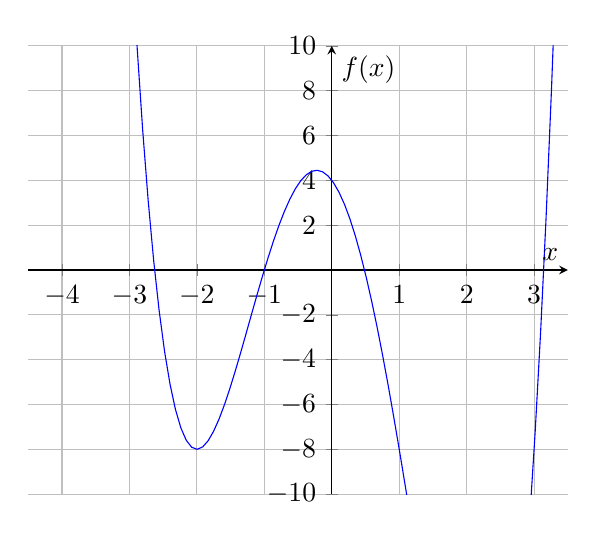
\begin{tikzpicture}
    \begin{axis}[
        xlabel={$x$},
        ylabel={$f(x)$},
        axis lines=middle,
        xmin=-4.5, xmax=3.5,
        ymin=-10, ymax=10,
        xtick={-4, -3, ..., 3},
        ytick={-10, -8, ..., 10},
        grid,
        samples=100
    ]
    \addplot[blue,domain=-4.5:3.5] {(x - 3)*(x - 1)*(x + 2)^2 - 8};
    \end{axis}
    \end{tikzpicture}
    \end{center}
    
    \item[\textbf{b)}] Three x-intercepts:
    
    To have three x-intercepts, we need to choose \(c = -4\).
    
    \begin{center}
    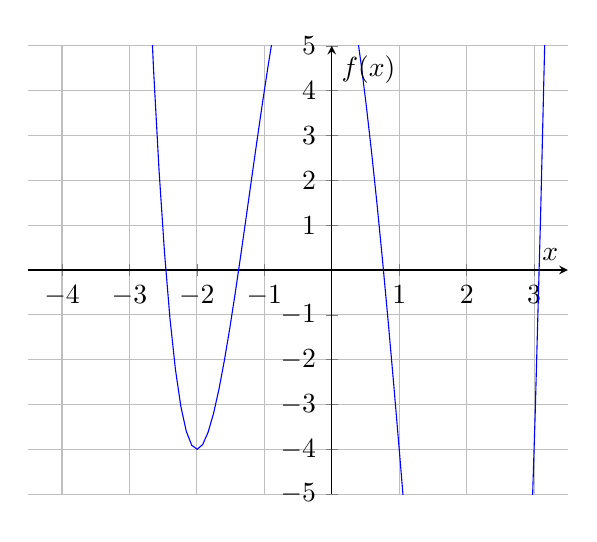
\begin{tikzpicture}
    \begin{axis}[
        xlabel={$x$},
        ylabel={$f(x)$},
        axis lines=middle,
        xmin=-4.5, xmax=3.5,
        ymin=-5, ymax=5,
        xtick={-4, -3, ..., 3},
        ytick={-5, -4, ..., 5},
        grid,
        samples=100
    ]
    \addplot[blue,domain=-4.5:3.5] {(x - 3)*(x - 1)*(x + 2)^2 - 4};
    \end{axis}
    \end{tikzpicture}
    \end{center}
    
    \item[\textbf{c)}] Two x-intercepts:
    
    To have two x-intercepts, we choose \(c = 3\).
    
    \begin{center}
    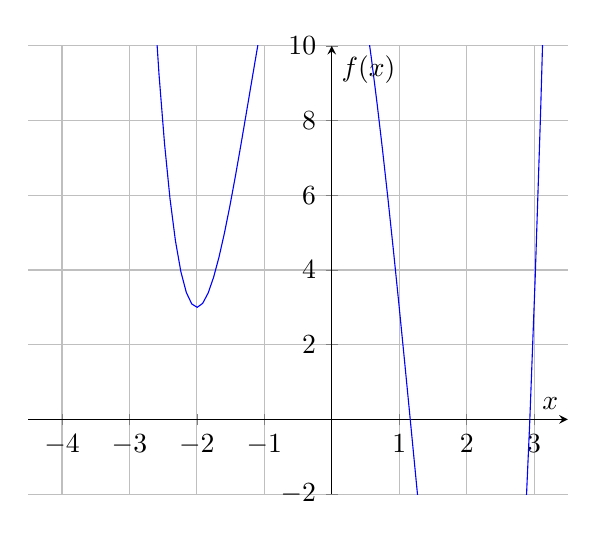
\begin{tikzpicture}
    \begin{axis}[
        xlabel={$x$},
        ylabel={$f(x)$},
        axis lines=middle,
        xmin=-4.5, xmax=3.5,
        ymin=-2, ymax=10,
        xtick={-4, -3, ..., 3},
        ytick={-2, 0, ..., 10},
        grid,
        samples=100
    ]
    \addplot[blue,domain=-4.5:3.5] {(x - 3)*(x - 1)*(x + 2)^2 + 3};
    \end{axis}
    \end{tikzpicture}
    \end{center}
    
    \item[\textbf{d)}] One x-intercept:
    
    To have one x-intercept, we choose \(c = 6\).
    
    \begin{center}
    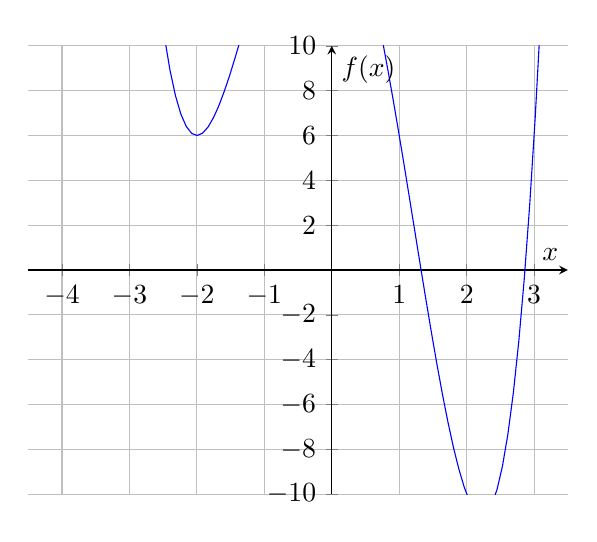
\begin{tikzpicture}
    \begin{axis}[
        xlabel={$x$},
        ylabel={$f(x)$},
        axis lines=middle,
        xmin=-4.5, xmax=3.5,
        ymin=-10, ymax=10,
        xtick={-4, -3, ..., 3},
        ytick={-10, -8, ..., 10},
        grid,
        samples=100
    ]
    \addplot[blue,domain=-4.5:3.5] {(x - 3)*(x - 1)*(x + 2)^2 + 6};
    \end{axis}
    \end{tikzpicture}
    \end{center}
    
    \item[\textbf{e)}] Zero x-intercepts:
    
    To have zero x-intercepts, we choose \(c = 8\).
    
    \begin{center}
    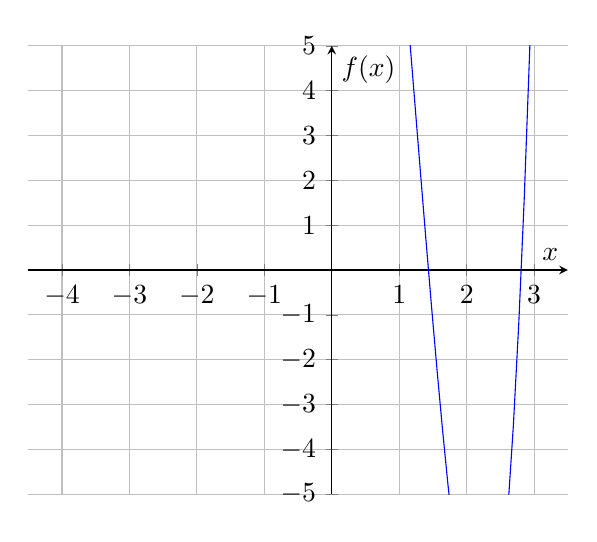
\begin{tikzpicture}
    \begin{axis}[
        xlabel={$x$},
        ylabel={$f(x)$},
        axis lines=middle,
        xmin=-4.5, xmax=3.5,
        ymin=-5, ymax=5,
        xtick={-4, -3, ..., 3},
        ytick={-5, -4, ..., 5},
        grid,
        samples=100
    ]
    \addplot[blue,domain=-4.5:3.5] {(x - 3)*(x - 1)*(x + 2)^2 + 8};
    \end{axis}
    \end{tikzpicture}
    \end{center}
\end{enumerate}

\end{itemize}
\end{document}